\section{Method}

\subsection{Overview}

LeWAM jointly predicts future video latents and robot actions using a single conditional flow-matching Diffusion Transformer~\cite{DiT, FlowMatching, esser2024scaling}, following the joint video-action denoising approach of ~\citet{DreamZero}, \citet{UWM}, and \citet{CosmosPolicy}. Rather than the VAE latents used by most other WAMs, our proposed method denoises video latents from a JEPA video encoder.

The model processes a sequence of three token groups: (1) \textbf{context video tokens} (clean), (2) \textbf{future video tokens} (noisy), and (3) \textbf{action tokens} (noisy), with a block-causal attention mask that enforces temporal ordering.
A frozen V-JEPA~2.1 encoder~\cite{vjepa2_1} provides the video representation used for both context and future ground truth. Additionally, a frozen SmolVLM2~\cite{SmolVLM2, SmolVLA} and an unfrozen state encoder provide visually-grounded language and state conditioning via cross-attention~\cite{GenTron}.

Figure~\ref{fig:arch} illustrates the full architecture.

[TODO: add model parameters to appendix (depth, model dimensions, action loss weight used in training, etc.)]

%---------------------------------------

\subsection{Video Encoder}

We use V-JEPA~2.1~\citep{vjepa2_1} ViT-B as our visual encoder, initialized from pretrained weights and frozen during training. The ViT-B variant was distilled from the main ViT-G model, reducing it to only 80 million parameters. 

All camera views are concatenated horizontally, then divided into spatial patches of size $16 \times 16$ and grouped into tubelets of temporal size 2, halving the temporal token count.
We use a crop size of $256 \times 256$ per input image in practice, producing a $16 \times 16$ token grid per camera per frame, although the use of 3D-RoPE interpolation~\cite{ThreeDRoPE} in both VJEPA2 and our DiT allows for this value to be changed at inference-time.

Given $C$ context frames and horizon $H$, the encoder produces context latents $\mathbf{z}_{0:C} \in \mathbb{R}^{H_p W_p \times D_{\text{enc}}}$ and future targets $\mathbf{z}_{C:H} \in \mathbb{R}^{H_p W_p \times D_{\text{enc}}}$, where $D_{\text{enc}} = 768$.

%---------------------------------------

\subsection{Visually Grounded Language Conditioning}

We use SmolVLM2-256M~\cite{SmolVLM2, SmolVLA} as our language encoder for its compact size and video pretraining, although the 500M variant can be used as a drop in replacement like in \citet{SmolVLA}. The VLM's vision encoder and connector are used to encode image or video context, which is prepended to the language token sequence before passing through the first $N$ language model layers. Similar to SmolVLA, instead of using only the hidden state after layer $N$, we store every intermediate hidden state $h_{i \in [1, N]}$, and have DiT block $i$ cross attend to the hidden state $h_i$.

During training, language conditioning is dropped with probability $p_{\text{drop}} = 0.15$ to enable classifier-free guidance at inference time~\cite{DreamZero}.

%---------------------------------------

\subsection{Joint Flow-Matching DiT}

Unlike some WAMs that use separate models for video and action prediction~\cite{MimicVideo, VLAJEPA, TRIWAM}, we adopt the joint denoising formulation of ~\citet{DreamZero}, \citet{UWM}, and \citet{CosmosPolicy},  predicting both future video latents and actions jointly in a single DiT. The input sequence is constructed by concatenating the context, future, and action tokens. Noise is added in the native action and encoder spaces ($D_{\text{action}}$ and $D_{\text{enc}}$) before projection to $D$ via separate linear layers.

\paragraph{DiT Block Structure.}
Each transformer layer consists of: (1) \textbf{block-causal self-attention} over the full token sequence with 3D-RoPE positional encoding~\cite{ThreeDRoPE, DreamZero, vjepa2_1} (see Appendix~\ref{attn_structure}), where video tokens receive $(t, h, w)$ position IDs and action tokens receive $(t, 0, 0)$; (2) \textbf{cross-attention} to proprioceptive state (encoded via a two-layer MLP) and language tokens from SmolVLM2; and (3) an \textbf{MLP} feedforward block. All sub-layers use adaLN-Zero~\citep{DiT} conditioning on the timestep embedding $\tau(t)$, with weights initialized to zero for stable early training.

\paragraph{Flow Matching Objective.}

Given a training sample with context latents $\mathbf{z}_{0:C}$, future targets $\mathbf{z}_{C:H}$, target actions $\mathbf{a}_{C:H}$, state $\mathbf{s}_{C-1}$, image $\mathbf{I}_{C-1}$, and language tokens $\mathbf{l}_{C-1}$, we sample noise $\boldsymbol{\epsilon}_z \sim \mathcal{N}(0, I)$, $\boldsymbol{\epsilon}_a \sim \mathcal{N}(0, I)$, and a shared timestep $t \sim \mathcal{U}[0, 1]$.
The noisy inputs are constructed via linear interpolation:
\begin{equation}
    \mathbf{z}_t = (1 - t)\,\boldsymbol{\epsilon}_z + t\,\mathbf{z}_{C:H}, \qquad \mathbf{a}_t = (1 - t)\,\boldsymbol{\epsilon}_a + t\,\mathbf{a}_{C:H}.
\end{equation}

The model predicts velocity fields $\hat{\mathbf{v}}_z, \hat{\mathbf{v}}_a = f_\theta(\mathbf{z}_t, \mathbf{a}_t, \mathbf{z}_{0:C}, t, \mathbf{s}_{C-1}, \mathbf{I}_{C-1}, \mathbf{l}_{C-1})$, and the flow matching loss is:
\begin{equation}
    \mathcal{L}_{\text{flow}} = \left\| \hat{\mathbf{v}}_z - (\mathbf{z}_{C:H} - \boldsymbol{\epsilon}_z) \right\|^2 + \lambda_a \left\| \hat{\mathbf{v}}_a - (\mathbf{a}_{C:H} - \boldsymbol{\epsilon}_a) \right\|^2,
\end{equation}
where $\lambda_a$ balances the video and action losses.

\paragraph{Inference}

At inference time, we sample initial noise for both video latents and actions and integrate the learned velocity field from $t = 0$ to $t = 1$ using Euler integration:
\begin{equation}
    \hat{\mathbf{z}}_{t+\Delta t} = \hat{\mathbf{z}}_t + \hat{\mathbf{v}}_z \cdot \Delta t, \qquad \hat{\mathbf{a}}_{t+\Delta t} = \hat{\mathbf{a}}_t + \hat{\mathbf{v}}_a \cdot \Delta t.
\end{equation}

The predicted actions are optionally smoothed using a Savitzky-Golay filter to remove high frequency noise left over from the denoising process~\cite{DreamZero}.

\paragraph{Action normalization.}
Actions and proprioceptive state are normalized using precomputed dataset statistics. Values are clipped to the 1st/99th percentiles and z-scored, preventing outliers from distorting the learning signal.

%---------------------------------------

\subsection{Training}

\begin{figure}[h]
    \centering
    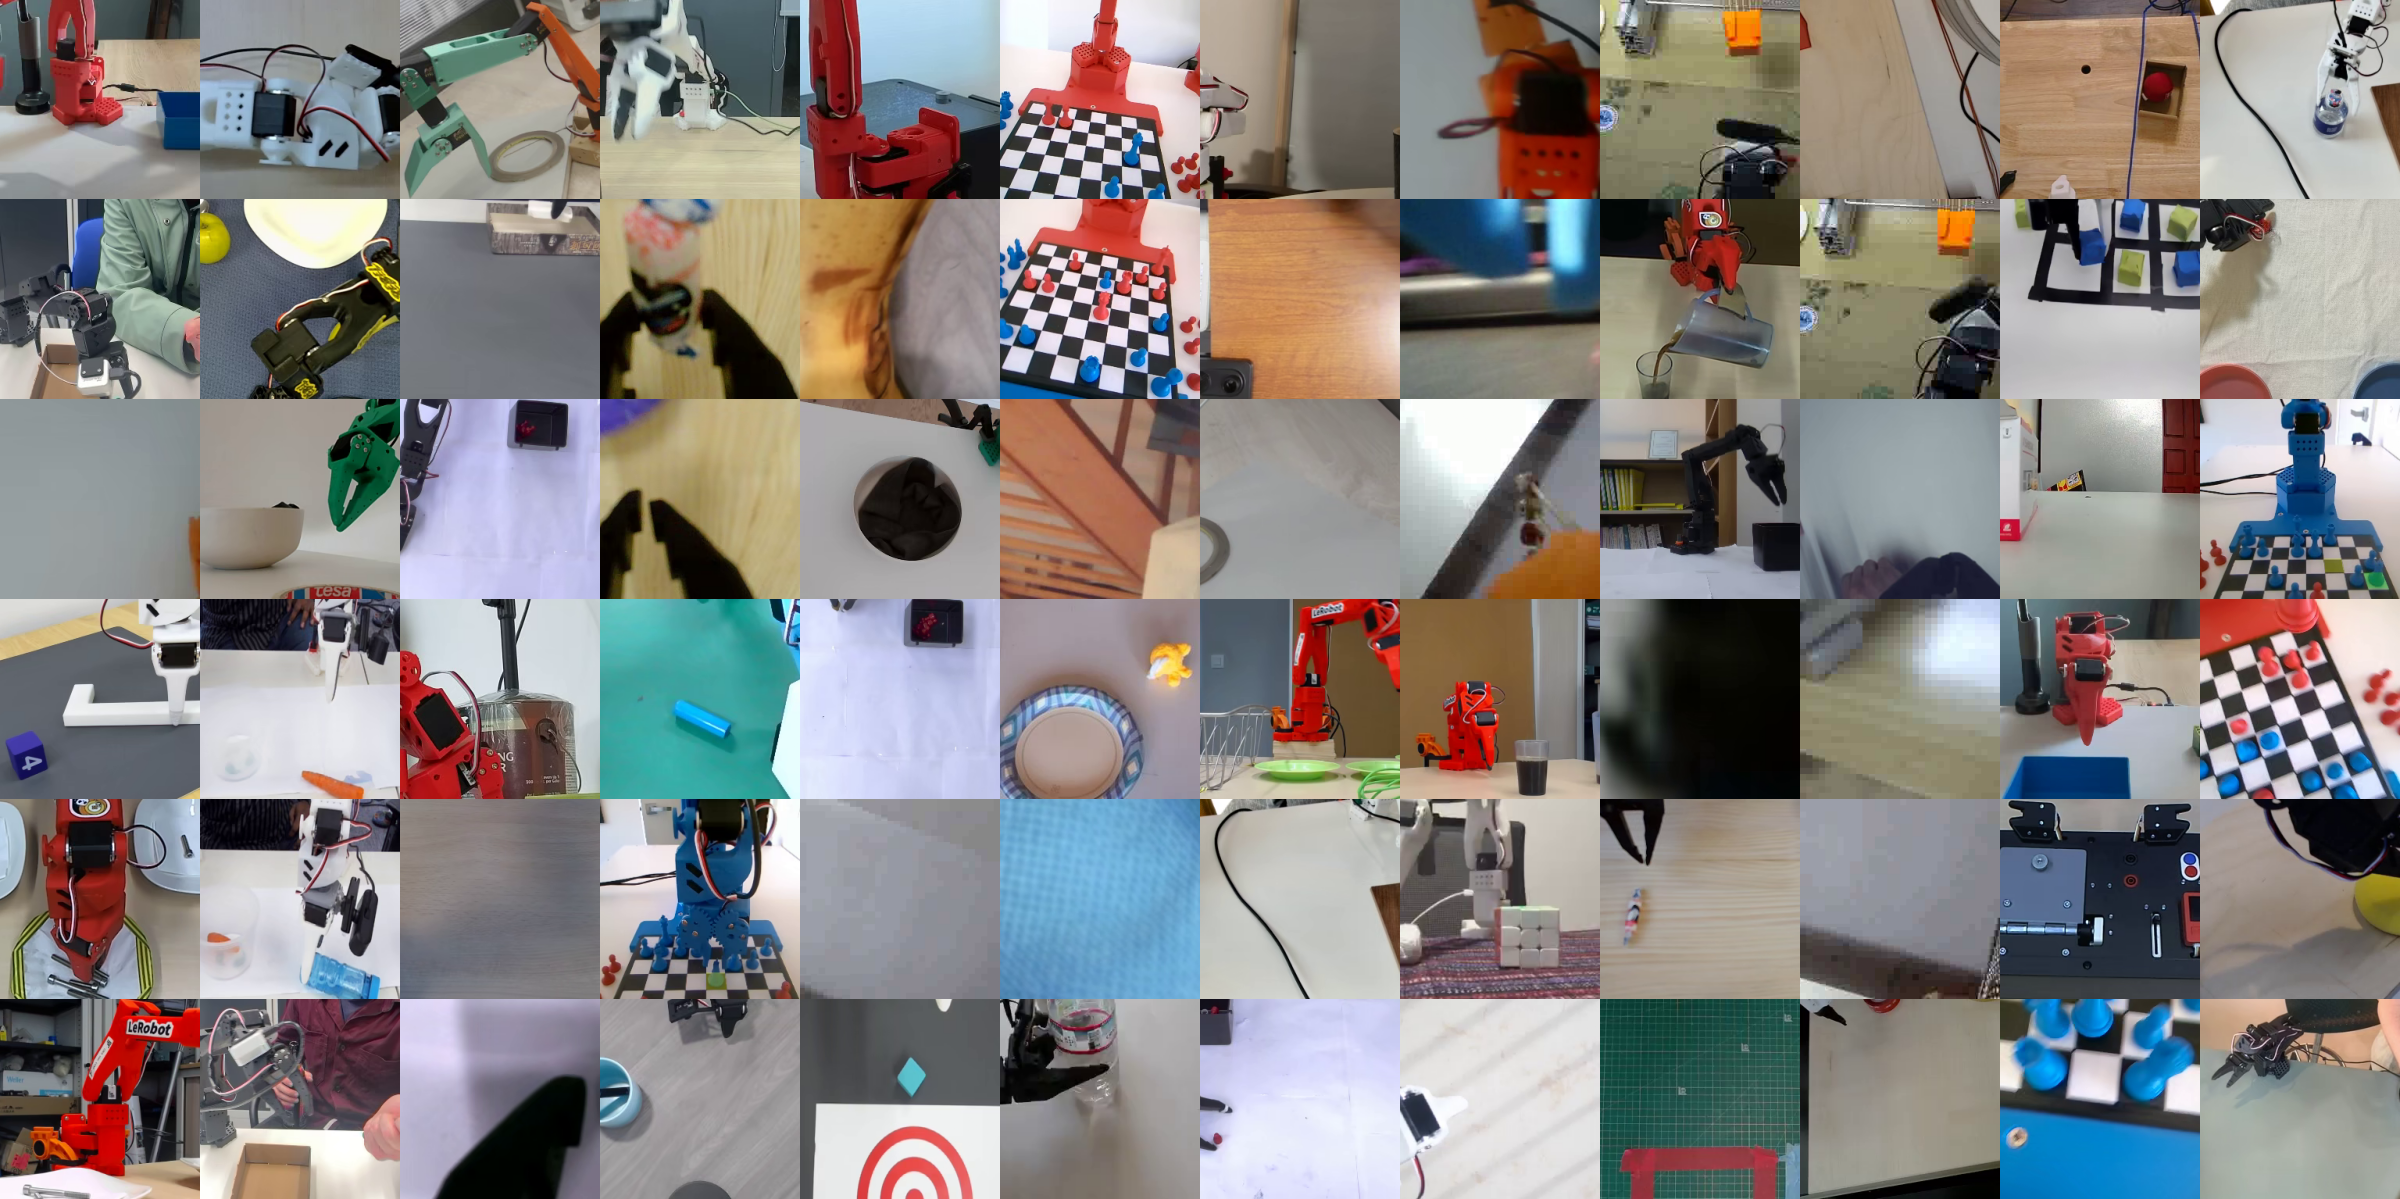
\includegraphics[width=\textwidth]{figures/generated/dataset_grid.png}
    \caption{A sample of episodes from the HuggingFaceVLA community dataset used for pretraining in SmolVLA\cite{SmolVLA} and our proposed method.}
    \label{fig:dataset}
\end{figure}

\paragraph{Robot pretraining data.}
We train on the open-source HuggingFaceVLA community dataset utilized in \citet{SmolVLA} (HuggingFace: \texttt{HuggingFaceVLA/community\_dataset\_v2}). The dataset is a collection of community-contributed robot manipulation demonstrations from the SO-101 and SO-100 low-cost arms, spanning 60 hours of in-the-wild data collected using the LeRobot framework~\cite{LeRobot}.

Most of the data preprocessing follows ~\citet{SmolVLA}, however new demonstrations were added in the second iteration of the dataset, prompting additional data preprocessing which was not done in the original SmolVLA project. Some added datasets did not match the SO-101/100 embodiments, and a handful of demonstrations had undescriptive task labels; such episodes were either manually deleted or relabeled. 

Additionally, the original dataset was published using the LeRobotDataset v2.1 format, which is deprecated. To better support modern tooling, we converted the entire to dataset to LeRobotDataset v3.0 and published it on HuggingFace (HuggingFace: \texttt{ehalicki/LeWAM\_community\_dataset})

\paragraph{Finetuning data.}
For our fine tuning experiments we collected [TODO: currently projecting ~200] demonstrations across 4 tasks using the SO-101 arm, similar to \citet{SmolVLA}. 

[TODO describe the tasks (pick and place, sorting, stacking)]

\paragraph{Training schedule}

[TODO: fill in once pre training and fine tuning schedules are finalized]

%---------------------------------------

[TODO: add a python pseudocode section like LeWorldModel]
